\chapter{Optimierung}
\section{Initialisierung}
Zu Beginn muss die Herde aller Elefanten in Clans aufgeteilt werden, wobei davon ausgegangen wird, dass jeder Clan eine feste Nummer an Tieren beinhaltet, genau einen Matriarchen hat und, dass mit jeder Generation eine feste Anzahl an männlichen Elefanten ihren Clan verlässt. 

\section{Clan-Update-Operator}
Jeder Clan hat einen Matriarchen, dem die Tiere folgen. Daher ist die neue Position $x_{new, ci, j}$ eines Elefanten $j$ in Abhängigkeit von seinem Clan $ci$ und der Position des zugehörigen Matriarchen $x_{best, ci}$ bestimmt (siehe \autoref{calcXNew}). 
\begin{equation}
    x_{new, ci, j} + \alpha \cdot (x_{best, ci} - x_{ci, j}) \cdot r
    \label{calcXNew}
\end{equation}
$x_{ci, j}$ stellt dabei die alte Position des Elefanten und $\alpha \in [0,1]$ einen Skalierungsfaktor, der den Einfluss des Matriarchen ausdrückt. Für $r$ gilt $r \in [0,1]$.\\
\\
Die Position des Matriarchen kann mit \autoref{calcXNew} nicht berechnet werden und es muss \autoref{calcXNewMatriarch} genutzt werden.
\begin{equation}
    x_{new, ci, j} = \beta \cdot x_{center, ci}
    \label{calcXNewMatriarch}
\end{equation}
Die Position des Matriarchen wird mittels der Position des zentralen Tieres $x_{center, ci}$ innerhalb des Clans $ci$ und $\beta \in [0,1]$ repräsentiert einen Skalierungsfaktor. $x_{center, ci}$ kann mittels \autoref{calcXCenter} berechnet werden.
\begin{equation}
    x_{center, ci, d} = \frac{1}{n_{ci}} \cdot \sum_{j=1}^{n_{ci}} x_{ci,j,d}
    \label{calcXCenter}
\end{equation}
Die Position des Tieres $x_{center, ci}$ ist zusätzlich abhängig von der Dimension $d$ mit $1 \leq d \leq D$ und der Anzahl der Tiere in einem Clan $n_{ci}$.

\section{Separierungs-Operator}
Der Separierungsprozess beschreibt das Verlassen der männlichen Elefanten des Clans beim Heranwachsen. Die Zahl der Mitglieder bleibt dabei jedoch gleich, die Elefanten werden lediglich ersetzt. Zur Optimierung der Annäherung an das Ziel wird dabei angenommen, dass der Elefant mit der schlechtesten Position ($x_{worst, ci}$) zum Ziel den Clan verlässt (siehe \autoref{calcXWorst}).
\begin{equation}
    x_{worst, ci} = x_{min} + (x_{max} - x_{min} + 1) \cdot rand
    \label{calcXWorst}
\end{equation}
$x_{max}$ und $x_{min}$ stellen die oberen bzw. unteren Grenzen der jeweiligen Dimension dar und $rand \in [0,1]$ eine Zufallszahl.\\
\\
In \autoref{eho_flowchart} ist der gesamte Ablauf des Algorithmus dargelegt. 



\begin{figure}[ht]
    \begin{center}
        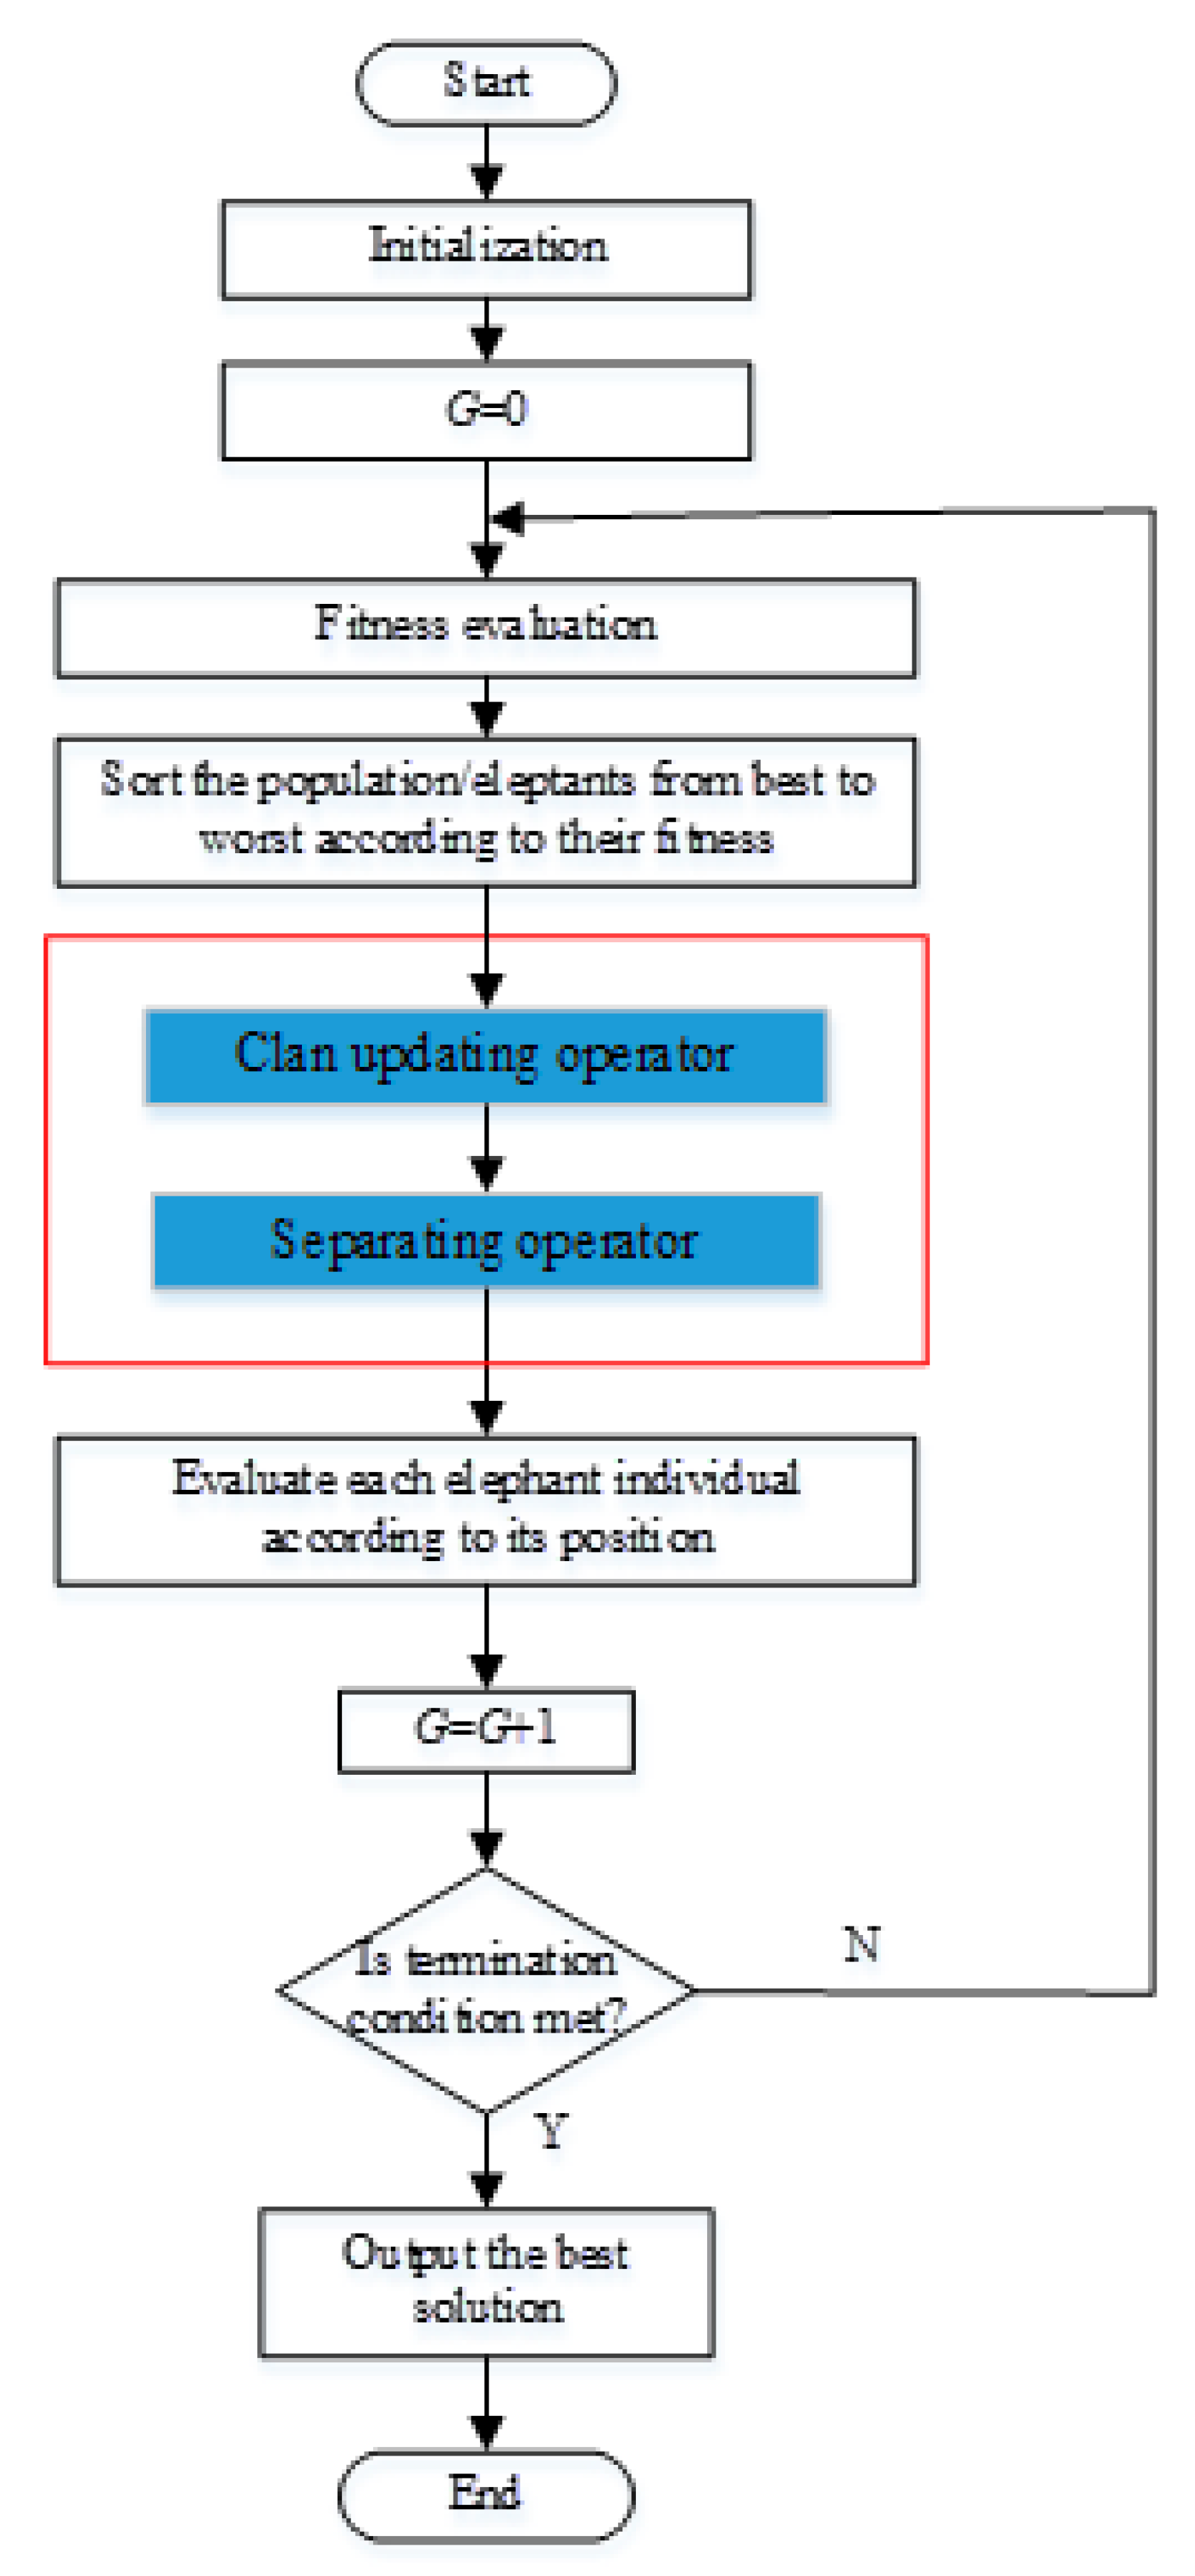
\includegraphics[width=0.5\textwidth]{assets/img/eho_flowchart.png}
        \caption[EHO Flowchart]{\cite[Li et al, S.4]{li_lei_alavi_wang_2020}}
        \label{eho_flowchart}
    \end{center}
\end{figure}

\begin{figure}[ht]
    \begin{center}
        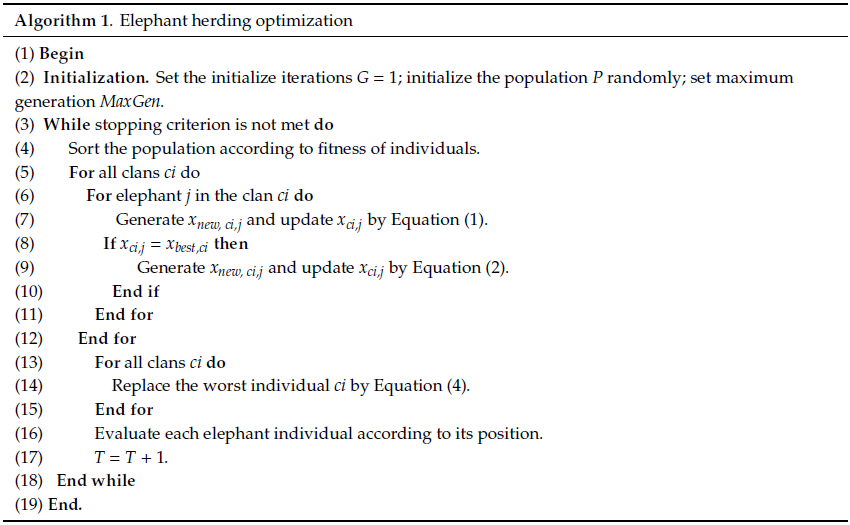
\includegraphics[width=0.9\textwidth]{assets/img/eho_pseudocode.PNG}
        \caption[EHO Pseudocode]{\cite[Li et al, S.5]{li_lei_alavi_wang_2020}}
        \label{eho_pseudocode}
    \end{center}
\end{figure}